\documentclass{acm_proc_article-sp}
\usepackage[utf8]{inputenc}
\usepackage[english]{babel}
\usepackage{minted}
\usepackage{lineno}
\usepackage{enumitem}
\usepackage{amsmath}
\usepackage{tikz}
\usepackage{caption}
\usepackage{subcaption}
\usepackage{epigraph}
\usepackage{multirow}
\usepackage{tabularx}
\usepackage{datetime}
\usepackage{catchfile}
\usepackage{hyperref}

\usepackage[backend=biber,style=ieee,sorting=nty,citestyle=numeric-comp,urldate=edtf]
{biblatex} \addbibresource{./papers/references.bib}

%%% Tooling %%%

%%%%%%%%%%%%%%%%%%%%%%%%%%%%%%%%%%%%%%%%%%%%%%%%%%%%%%%%%%%%%%%%%%%%%%
% LaTeX Overlay Generator - Annotated Figures v0.0.1
% Created with http://ff.cx/latex-overlay-generator/
%%%%%%%%%%%%%%%%%%%%%%%%%%%%%%%%%%%%%%%%%%%%%%%%%%%%%%%%%%%%%%%%%%%%%%
%\annotatedFigureBoxCustom{bottom-left}{top-right}{label}{label-position}{box-color}{label-color}{border-color}{text-color}
\newcommand*\annotatedFigureBoxCustom[8]{\draw[#5,thick,rounded corners] (#1) rectangle (#2);\node at (#4) [fill=#6,thick,shape=circle,draw=#7,inner sep=2pt,font=\sffamily,text=#8] {\textbf{#3}};}
%\annotatedFigureBox{bottom-left}{top-right}{label}{label-position}
\newcommand*\annotatedFigureBox[4]{\annotatedFigureBoxCustom{#1}{#2}{#3}{#4}{white}{white}{black}{black}}
\newcommand*\annotatedFigureText[4]{\node[draw=none, anchor=south west, text=#2, inner sep=0, text width=#3\linewidth,font=\sffamily] at (#1){#4};}
\newenvironment {annotatedFigure}[1]{\centering\begin{tikzpicture}
\node[anchor=south west,inner sep=0] (image) at (0,0) { #1};\begin{scope}[x={(image.south east)},y={(image.north west)}]}{\end{scope}\end{tikzpicture}}
%%%%%%%%%%%%%%%%%%%%%%%%%%%%%%%%%%%%%%%%%%%%%%%%%%%%%%%%%%%%%%%%%%%%%%

\newcommand\footnoteref[1]{\protected@xdef\@thefnmark{%
\ref{#1}}\@footnotemark} \makeatother

\CatchFileDef{\HEAD}{../.git/refs/heads/master}{}
\newcommand{\gitrevision}{%
\StrLeft{\HEAD}{7}%
}

\newcommand{\code}[1]{\texttt{#1}}

\setlength{\paperheight}{11in} \usetikzlibrary{automata,arrows,positioning,calc,fit}

% \linenumbers

%%% Textual %%%

\newcommand{\thesistitle}{Debugging Data-Flows in Reactive Programs}
\hypersetup{pdftitle={\thesistitle}}

\hyphenation{Ob-serv-ables}
\hyphenation{Marble}
\hyphenation{Diagrams}
\hyphenation{Java-Script}
\hyphenation{RxFiddle}

\newcommand{\printfdebugging}{{\code{printf}-debugging}}
\newcommand{\NodeJS}{{Node.js}}


\title{\thesistitle}
\numberofauthors{3}
\author{
    \alignauthor Herman Banken\\
    \affaddr{Delft University of Technology, The Netherlands}\\
    \begin{email}{hermanb@ch.tudelft.nl}
    \end{email}
    \alignauthor Georgios Gousios\\
    \affaddr{Delft University of Technology, The Netherlands}\\
    \begin{email}{g.gousios@tudelft.nl}
    \end{email}
    \alignauthor Erik Meijer\\
    \affaddr{Delft University of Technology, The Netherlands}\\
    \begin{email}{h.j.m.meijer@tudelft.nl}
    \end{email}
}
\begin{date}{\today}\end{date}

\begin{document}

\begin{minipage}[t]
    [0.99\textheight]{0.99\textwidth} %\begin{titlepage}
    \begin{center}
        \vspace*{1cm}

        \Huge \textbf{\thesistitle}

        \large
        \vspace{0.5cm} by
        \vspace{0.5cm}

        \Large \textbf{Herman Banken}\\
        \normalsize born in Woerden, The Netherlands

        \vspace{1cm}
        \vfill

        to obtain the degree of Master of Science\\
        at the Delft University of Technology,\\
        to be defended publicly on Wednesday July 5th, 2017 at 4:00 PM.

        \vspace{0.8cm}

        \begin{tabular}{l l l}
            Student number:   & \multicolumn{2}{l}{4078624} \\
            Project duration: & \multicolumn{2}{l}{September 12, 2016 - June 30, 2017} \\
            Thesis committee: & Prof. Dr. H.J.M. Meijer, & TU Delft \\
                              & Dr. G. Gousios,          & TU Delft \\
                              & Prof. Dr. A van Deursen, & TU Delft \\
                              & Joost de Vries,          & Ordina
        \end{tabular}

        \vspace{0.8cm}

        An electronic version of this thesis is available at \url{http://repository.tudelft.nl}.

        \begin{minipage}{6in}
            \centering
            $ \vcenter{\hbox{
\includegraphics[width=0.4\textwidth]{images/logo.pdf}}}
            $ \hspace*{.2in} $ \vcenter{\hbox{
\includegraphics[width=0.4\textwidth]
            {images/codestar.pdf}}} $
        \end{minipage}

        \small Version as of {\today} at \currenttime, Git version
        \gitrevision.

    \end{center}
    %\end{titlepage}
\end{minipage}


\maketitle \thispagestyle{empty}

% Ignore pagecounter from frontmatter
\setcounter{page}{1}

\begin{abstract}
    Reactive Programming is a way of programming designed to provide
developers with the right abstractions for creating systems that use
streams of data.  Traditional debug tools lack support for the
abstractions provided, causing developers to fallback to the most
rudimentary debug tool available:  \printfdebugging{}.

In this work, we design a visualization and debugging tool for Reactive
Programming, that aids comprehension and debugging of reactive systems,
by visualizing the dependencies and structure of the data flow, and the
data inside the flow.  We present RxFiddle, a platform for the
visualization as well as the required instrumentation for RxJS in the
ReactiveX-family of Reactive Programming libraries.  Evaluation based on
an experiment with 111 subjects, shows that RxFiddle can outperform
traditional debugging in terms of debug time required.

\end{abstract}

%\category{H.4}{Information Systems Applications}{Miscellaneous}
%\category{D.2.8}{Software Engineering}{Metrics}[complexity measures, performance measures]
\begin{keywords}{
reactive programming,
debugging,
visualization,
program comprehension
}\end{keywords}

% Stanford writing guide http://cs.stanford.edu/people/widom/paper-writing.html

%% Use Arabic numerals for the page numbers of the chapters.
\mainmatter

\section{Introduction}

Software often needs to respond to external events and data flows.
Consider for example software in interactive applications, for desktops,
web and mobile phones, in graphics and in processing sensor data from
phones or IoT-devices.  Traditionally, handling these asynchronous
events was done using the \emph{Observer design pattern}~\cite{johnson1995design}
or \emph{callback functions}~\cite{gallaba2015don}.  Using these
patterns, the system consuming the data does not have to block waiting
for methods to return, but instead receives a notification event when
data is available.  While these patterns decouple the consumer from the
producer of the data, they typically lead to dynamic registration, side
effects in the consumers, and inversion of control~\cite{salvaneschi2014empirical,edwards2009coherent}.

Reactive Programming (RP) is an alternative to these patterns for event
driven computation.  RP defines event streams as lazy collections and
provides operators that allow developers to deal with the complications
of asynchronous event handling.  It offers declarative and concise
syntax for composing streams of data, to express the complex reactive
behavior of these applications.  RP started in academia in the form of
Functional Reactive Programming (FRP)~\cite{elliott1997functional,elliott2009push,czaplicki2013asynchronous,maier2010deprecating,meyerovich2009flapjax},
but in recent years the use of RP has exploded.  Languages such as Elm~\cite
{czaplicki2012elm} and libraries such as Reactor~\cite{Gutierrez2017},
Akka~\cite{klangakka} and Rx~\cite{meijer2010subject} are being used by
companies like Netflix, Microsoft and Google, to build highly responsive
and scalable systems.  Front-end libraries like AngularJS, that use RP
in their foundations, are used by many large sites (9.1\% of Quantcast
Top 10k websites%
%URL to long for hbox; https://trends.builtwith.com/javascript/Angular-JS.
\footnote{\url{{https://trends.builtwith.com/}}, accessed 2017-06-20}).
Developers and companies alike attempted to standardize ``Reactive
Programming'' in the form of the Reactive Manifesto~\cite{boner2014reactive}.

While reactive programs might be more declarative and concise, RP does
not work well with traditional interactive debuggers, shipped with most
IDE\'s~\cite{salvaneschi2016debugging}.  RP borrows from Functional
Programming (FP) for its abstractions, its laziness and advocating the
use of ``pure'' lambda functions.  Those features contribute to a
control flow that is hidden inside the RP implementation library and
lead to non-linear execution of user code.  This results in not useful
stack traces, while breakpoints do not help either, since relevant variables
are frequently not in scope.  Furthermore, using a low level debugger makes
it harder to interact with the high level abstractions that RP provides.
Compared to imperative programming, there is limited scientific
knowledge regarding how developers debug reactive programs.  Traditional
imperative program debugging practices~\cite{beller2017behavior} do not
apply to RP~\cite{salvaneschi2016debugging}.

In this work we address the issue of RP debugging by designing and
implementing a high level debugger called RxFiddle for a popular version
of RP, namely Reactive Extensions (Rx).  RxFiddle (1) provides an
overview of the dependencies in the data flow, (2) enables a detailed
insight in the data flow and the timing of individual events, and (3)
allows developers to trace values back through the data flow.  To guide
our design we conducted interviews among professional developers.  After
building RxFiddle, we validated it with a user experiment.  The results
show that RxFiddle can help developers debug RP data flows faster.

To steer the research, we formulate the following research questions:

\begin{description}
    \item[RQ1]
        How do developers debug RP?  \\
        Before we design tools it is important to understand the
        problems arising in the the current state~\cite{singer2010examination}.
        Anecdotal evidence by a number of resources%
        \footnote{%
        \label{foot:contribdays}http://contributordays.com/contributor-days/rxjs}%
        \footnote{https://staltz.com/how-to-debug-rxjs-code.html}
        suggests that debugging RP is difficult.

    \item[RQ2]
        How can we design a tool that helps developers debug RP?  \\
        By examining the results of RQ1, the limitations of traditional
        debuggers and the opportunities that RP programs offer in terms
        of structure and explicit dependencies between data flows, we
        design a novel RP debugger.

    \item[RQ3]
        Can specialized RP debuggers speed up comprehension \&
        debugging?  \\
        To validate our design and examine whether specialized tooling
        can improve the experience we measure the speed and correctness
        of comprehension in an experiment.

\end{description}


\section{Background: RP}
\label{background}
\label{nutshell}

Reactive Programming (RP) is a declarative programming paradigm for working with streams of input data. 
According to the first definition\footnote{
``Reactive programs [..] maintain a continuous interaction with their environment, at a speed which is determined by the environment, not the program itself.''~\cite{berry1989real}
} a reactive program must interact with the environment ``at a speed which is determined by the environment''.
Conceptually, when a reactive program is run, it sets up a data pipeline and waits until input arrives when the environment changes.
Reactive Programming languages and libraries provide developers with a set of abstractions and methods to create such programs.

The programming paradigm of Reactive Programming is implemented by multiple languages and libraries. 
Many RP implementations share a notion of a collection that abstracts over \emph{time}, in contrast to \emph{space} like standard collections.
This collection comes in different flavors, 
such as Observable (Rx~\cite{meijer2010subject}), 
Signal (Elm~\cite{czaplicki2012elm}), 
Signal/Event (REScala~\cite{salvaneschi2014rescala}) or 
Behavior/Event (FRP~\cite{elliott1997functional}).
The implementations differ in the precise semantics of their collections, their execution model (push/pull), and the set of available operators.  
In this paper, we focus on the Rx formulation, but our work is applicable to other RP implementations to some extend. 

Understanding how we arrive at our visualization requires a minimal understanding of Rx.
Rx introduces two basic types \emph{Observable} and \emph{Observer}. Observables define the data flow and produce the data while Observers receive the data, possibly moving the data further down the stream. Figure \ref{sample1} shows a very basic example of an ``in situ'' data flow in Rx. Initially, an Observable is created, here using the static \code{of} method, then dependent Observables are created using the \code{map} and \code{filter} methods on the Observable instance. Finally we \code{subscribe} to start the data flow and send the data in the flow to the console.

\begin{figure*}[ht!]
\centering

\begin{subfigure}[t]{\columnwidth}
	\inputminted[tabsize=2]{javascript}{listings/sample1.js}	
	\par\bigskip
	\caption{Rx code example}
	\label{sample1}
	\par\medskip
	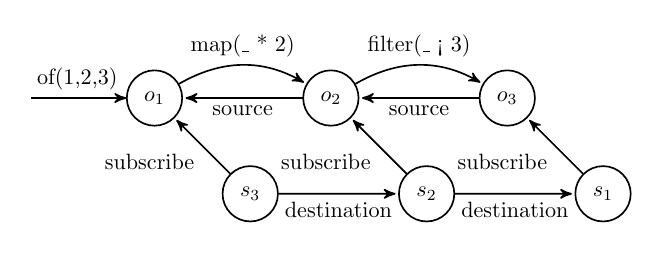
\begin{tikzpicture}[->,>=stealth',shorten >=1pt,auto,node distance=2.8cm,
                    semithick,scale=0.8, every node/.style={scale=0.8}]
  \tikzstyle{every state}=[]

  \node[state] (A)                    {$o_1$};
  \node[state] (B) [right of=A]       {$o_2$};
  \node[state] (C) [right of=B]       {$o_3$};

  \node[state] (X) [below right =1cm of A] {$s_3$};
  \node[state] (Y) [right of=X]            {$s_2$};
  \node[state] (Z) [right of=Y]            {$s_1$};

  \path (B) edge   node {source}                   (A)
        (C) edge   node {source}                   (B)
        (A) edge [bend left] node {map(\_ * 2)}    (B)
        (B) edge [bend left] node {filter(\_ < 3)} (C)
        (X) edge   node[below] {destination}       (Y)
        (Y) edge   node[below] {destination}       (Z)
        (Z) edge   node {subscribe}                (C)
        (Y) edge   node {subscribe}                (B)
        (X) edge   node {subscribe}                (A);

  \draw[<-] (A) -- node[above] {of(1,2,3)} ++(-2cm,0);
  %\draw[<-] (Z) -- node[below] {subscribe} ++(2cm,0);

\end{tikzpicture}

	\caption{Rx graph example}
	\label{chaincreate}
\end{subfigure}
\begin{subfigure}[t]{\columnwidth}
	\inputminted[tabsize=2]{javascript}{listings/sample3.js}	
	\caption{Higher order flatMap operation}
	\label{sample3}
	\par\medskip
	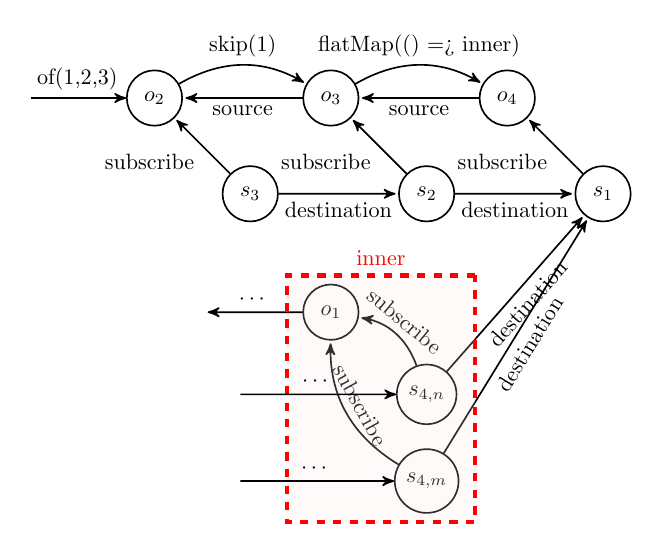
\begin{tikzpicture}[->,>=stealth',shorten >=1pt,auto,node distance=2.8cm,
                    semithick,scale=0.8, every node/.style={scale=0.8}]
  \tikzstyle{every state}=[]

  \node[state] (A)                    {$o_2$};
  \node[state] (B) [right of=A]       {$o_3$};
  \node[state] (C) [right of=B]       {$o_4$};

  \node[state] (X) [below right =1cm of A] {$s_3$};
  \node[state] (Y) [right of=X]            {$s_2$};
  \node[state] (Z) [right of=Y]            {$s_1$};
  
  \node[state] (F) [below =2cm of B]              {$o_1$};
  \node[state] (P) [below =1.8cm of Y] {$s_{4,n}$};
  \node[state] (Q) [below =0.3cm of P]       {$s_{4,m}$};

  \path (B) edge   node {source}                   (A)
        (C) edge   node {source}                   (B)
        (A) edge [bend left] node {skip(1)}    (B)
        (B) edge [bend left] node {flatMap(() => inner)} (C)
        (X) edge   node[below] {destination}       (Y)
        (Y) edge   node[below] {destination}       (Z)
        (Z) edge   node {subscribe}                (C)
        (Y) edge   node {subscribe}                (B)
        (X) edge   node {subscribe}                (A)
        
        (P) edge [bend right]  node[sloped,above] {subscribe}   (F)
        (P) edge   node[sloped,below] {destination} (Z)
        (Q) edge [bend left]  node[sloped,above] {subscribe}   (F)
        (Q) edge   node[sloped,below] {destination} (Z);
  
%  \node[draw=none] (K) at ($ (P) + (-4:-3) $){$\cdots$};
%  \node[draw=none] (M) at ($ (Q) + (-4:-3) $){$\cdots$};  
        
  % https://tex.stackexchange.com/questions/75497/automata-container-box
  \node [draw=red, label={\color{red}inner}, fit=(F) (P) (Q), inner sep=0.5cm,dashed, ultra thick, fill=red!10, fill opacity=0.2] {};
  %\node [draw=blue, fit= (G) (Q) (M), inner sep=0.5cm,dashed, ultra thick, fill=blue!10, fill opacity=0.2] {};

  % https://tex.stackexchange.com/questions/160643/ellipsis
  \draw[<-] (A) -- node[above] {of(1,2,3)} ++(-2cm,0);
  \draw[->] (F) -- node[above] {$\cdots$} ++(-2cm,0);
  \draw[<-] (P) -- node[above] {$\cdots$} ++(-3cm,0);
  \draw[<-] (Q) -- node[above] {$\cdots$} ++(-3cm,0);

\end{tikzpicture}

	\caption{Higher order Rx graph example}
	\label{chainhigher}
\end{subfigure}

\caption{Samples of Rx Observables}

\end{figure*}

\paragraph{Assembly} It is important to note that Observables are lazy; initially they only specify the blueprint of a data flow. 
Creating this specification is called the \emph{assembly} phase. In the code sample of Figure \ref{sample1} the assembly phase consists of the calls to \code{of}, \code{map} and \code{filter}, creating respectively Observables $o_1$, $o_2$ and $o_3$ from Figure \ref{chaincreate}.

\paragraph{Subscription} When the \code{subscribe} method of an Observable is called, the data flow is prepared by recursively subscribing up the stream: every subscribe call creates an \emph{Observer}, that is passed to the input Observable, which again subscribes an Observer to its input Observable, until finally the root Observables are subscribed to. We call this the \emph{subscription} phase. In Figure \ref{sample1} inside the single \code{subscribe} call Observer $s_1$ from Figure \ref{chaincreate} is created and passed to $o_3$, which in turn will recursively subscribe to $o_2$ with a new Observer $s_2$ with destination $s_1$, until the full chain is subscribed.

\paragraph{Runtime} After the root Observables are subscribed to, they can start emitting data. This is the \emph{runtime} phase. Depending on the nature of the Observable this might attach event listeners to UI elements, open network connections or start iterating over a list of elements. Events are pushed to $s_3$, to $s_2$ and finally to $s_1$ which calls \code{console.log} in Figure \ref{sample1}. 

Rx identifies three types of events that can occur during the runtime phase: \emph{next}, \emph{error} and \emph{complete}-events. Next-events contain the next value in the flow, an error-event encapsulates an error and is a unsuccessful termination to a stream, while a complete-event denotes the successful termination of the stream. There are restrictions on their order: a Observable may first emit an unlimited amount of next-events, and then either an error or a complete event. Observables do not need to emit any next-events, and do not need to terminate.

More complex programs feature operators that merge Observables\footnote{
	\code{concat}, \code{merge}, \code{combineLatest}, \code{zip}
}, split Observables\footnote{
	\code{partition}, or through sharing with \code{share} or \code{publish}
} or handle higher order Observables\footnote{
	\code{flatMap}, \code{mergeMap}, \code{concatMap}
}, resulting in more complex graphs. While merging and splitting happens on an Observable level (the \code{source} property still points to the one or more dependencies) higher order Observable flattening manifests only in Observer structure (there is no reference between the Observables). Figure \ref{chainhigher} shows this with an (abbreviated) \code{inner} Observable that is subscribed twice (for both values $2$ and $3$, value 1 is skipped), resulting in two identical data flows over $o_1$. The data flow through $s_{4,n}$ and $s_{4_m}$ is pushed into $s_1$, flattening the data flow. 

\begin{figure}[t]
\centering
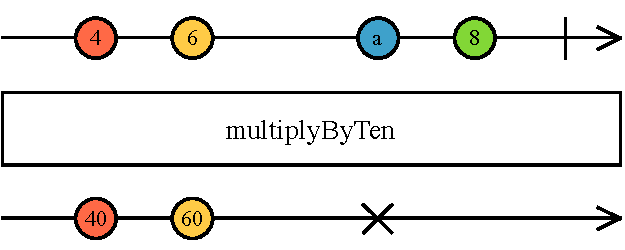
\includegraphics[width=\columnwidth]{images/marble-diagram.pdf}
\caption{Marble Diagram}
\label{marblediagram-image}
\end{figure}

\paragraph{Marble Diagram}
\label{marblediagram}
The term \textit{Marble Diagram} comes from the shape of the glyps in the images used to explain Rx in the official documentation. An example is shown in Figure~\ref{marblediagram-image}.
The diagrams contain one or more timelines containing the events that enter and leave Observables. 
Next-events are typically represented with a circle, an error-event with a cross and a complete-event with a vertical line.
Developers can see from the diagram how operators work by inspecting the difference between the timelines, 
where events might be skipped, added, transformed or delayed. 
Mapping time on the x-axis provides insight that is missing when inspecting only a single time slice. 

\section{Research Design} % page 212 of Creswell-Cap-10.pdf
To answer our research questions, we employ a three-phase Sequential
Exploratory Strategy, one of the mixed methods research approaches~\cite
{creswell2013research,hanson2005mixed}, as shown in Table~%
\ref{research-methods}.  First, we interview professional developers and
review available documentation (RQ1) to form a understanding about
current debugging practices, second we apply this understanding to
design a debugger and implement it to test its feasibility (RQ2),
finally we validate the debugger using an experiment (RQ3).

\begin{table}[t]
    \centering
    \begin{tabularx}{\columnwidth}
        {lllX}
        \hline
        \textbf{} & \textbf{Method} & \textbf{Focus} \\
        \hline
        \multirow{2}{*}{RQ1} & Interview & What are current practices \\
        & Literature & What is recommended \\
        \multirow{2}{*}{RQ2} & Design & What can a RP debugger show \\
        & Implement & Extract meta information from Rx \\
        RQ3 & Experiment & Quantification of effect on debugging \\
        \hline
    \end{tabularx}
    \caption{Research Methods used in the study}%
    \label{research-methods}
\end{table}

\iffalse \todo{ qualitive data quantitive design, implemented, tested
with real developers buzz words:  mixed methods, grounded theory }
\fi


\section{RP Debugging practices}%
\label{section-practices}

%\todo{alternative section titles: Evaluating motivation / collecting empirical evidence / case study}
To validate the need for better tools we must first understand how
existing tools are used (RQ1).  We interview developers, as we want to
explore and understand the current practices, instead of using an
experiment or survey to test a particular hypothesis.  The questions
were semi-structured.  We first established a general understanding of
the experience of the subjects.  Then we asked several open questions
regarding use of RP, how subjects debug RP and test RP.  Table%
\ref{interview-questions} lists the questions used as a guideline for
the interviews.

\begin{table*}[t]
    \centering
    \begin{tabular}{llc}
        \hline
                      & \textbf{Question}                       &  \\ 
        \hline
        Q1            & Explain your (professional) experience. & \multicolumn{1}{c}{\multirow{5}{*}{\begin{tabular}[c]{@{}c@{}}Context, \\ 
        understanding \\ 
        subjects
    \end{tabular}}} \\
    Q2  & Assess your experience on a scale from beginner to expert.
    & \multicolumn{1}{c}{} \\
    Q3  & Explain your (professional) reactive programming experience.
    & \multicolumn{1}{c}{} \\
    Q4  & Assess your RP experience on a scale from beginner to expert.
    & \multicolumn{1}{c}{} \\
    Q5  & Did you refactor or rework RP code?   & \multicolumn{1}{c}{}
    \\
    \hline
    Q6  & Did you and how did you test or verify the workings of RP
    code?       & \multirow{5}{*}{Content questions} \\
    Q7  & Did you and how did you debug RP code?        & \\
    Q8  & Did you and how did you use documentation on RP?      & \\
    Q9  & What difficulties did you experience with RP?         & \\
    Q10 & What is your general approach to understand a piece of Rx?
    & \\
    \hline
\end{tabular}
\caption{Interview questions}%
\label{interview-questions}
\end{table*}

Five developers with professional programming experience ranging from 4
to 12 years where interviewed.  The first four developers (D1-D4) work
in Company A, which builds mostly reactive systems~\cite{boner2014reactive}
using various RP solutions, and developers range from a month to over a
year of Rx experience.  The fifth developer (D5) works in Company B, and
is concerned with building and maintaining a large scale distributed
server application, that uses Rx to handle asynchronous events.

\subsection{Interviews} In the following paragraphs we discuss the
results of Q6-Q10 in detail.  Not every subject answered each question
in the same amount of detail, so we discuss the answers that provide
meaningful insights in the current practice.

\paragraph{Testing} Of the 4 subjects of Company A, none performed tests
specifically for Rx logic.  \emph{``Just running the application''}, is
enough according to D3, saying that they only test the business logic in
their application and consider the Rx code as ``glue''' which either
works or does not work.  In contrast, D5 and his team at Company B
extensively tests their application using the Rx' built-in test
facilities like ``marble tests'' and the \code{TestScheduler}~\cite{reactivex}.
Using tests, the subject \emph{confirms his believes about the behavior}
of the chain of operators, and tests also help later on when refactoring
code.

\paragraph{Debugging} All subjects independently mention using temporary
\printfdebugging{} statements (\code{console.log} in JavaScript).
Subjects use \printfdebugging{} to \emph{``add more context''} (D1) to
their debug sessions.  Printing which values flow through the flow
allows them to \emph{``quickly reason what happens''} (D3).  Breakpoints
are only used when the project requires costly recompilation otherwise (D1).
Existing debuggers often can not be used to inspect the life-cycle of
Observables (subscription and disposal), as these occurrences are not
normally defined in user code and would require breakpoints in library
code, like the \code{subscribe}-method, which is used by all class
instances of Observable.  This debugging inside the Rx library was
described as \emph{``painful''}, by D2 when using the Node.js debugger
to step through the inners of Rx.  Alternatives used by our subjects are
(1) creating a \emph{custom \code{debug} operator} which prints these
life-cycle events (D5) or (2) creating custom Observables (\code{Observable.create})
with \emph{custom subscribe and dispose methods}, inserted at the
beginning of the chain, that print upon their usage (D2, D5).  While
\printfdebugging{} and breakpoints are useful in various degrees when
executing a single Observable chain, these methods both become
considerably more difficult and \emph{``overview is easily lost''} when
executing multiple chains concurrently (D3, D5).

\paragraph{Documentation} Subjects give different reasons to visit the
documentation, but the most common reason is to \emph{``find an operator
for what I need''} (D1).  They feel that there might be an operator that
precisely matches their needs, however knowing all operators by heart is
not common (the Rx's Observable API has 28 static methods and 114
instance methods), therefore subjects sometimes end up doing an
extensive search for some specific operator.  Another reason to visit
the documentation is to \emph{comprehend how operators in existing code
work}.  For this subjects use the marble diagrams at \href{http://rxmarbles.com}
{RxMarbles.com}~\cite{rxmarbles} (D2, D5), the RxJS 4 documentation at
\href{https://github.com/Reactive-Extensions/RxJS/blob/master/doc/} {GitHub}
(D2, D5), the RxJS 5 documentation at \href{http://reactivex.io/rxjs} {ReactiveX.io}~\cite
{reactivex} (D1, D4, D5) and the online book \href{http://introtorx.com}
{IntroToRx.com}~\cite{introtorx} (D4).  D1 specifically mentions the
need for more examples in the documentation.

\paragraph{Difficulties experienced} The IDE does not help with
developing Rx (D2, D4); according to D4 \emph{``Rx is more about timing
than about types''}, and \emph{``You miss some sort of indication that
the output is what you expect''}.  It is not allways clear what happens
when you execute a piece of code, ``mostly due to Observables sometimes
being lazy'' (D2).  Flows are clear and comprehensible in the scope of a
single class or function, but for application wide flows it becomes
unclear (D3, D4 and D5).  D3 mostly used RxScala and mentions that
creating micro services helps in this regard.  D1 mentoins that \emph{``you
need to know a lot as a starting {\lbrack}RxJS{\rbrack} developer''},
giving the example of the many ways to cleanup and \code{unsubscribe},
which he did manually initially.  D1 used both logging while analyzing
existing code and learning to overcome inexperience.

\paragraph{Approach to understanding} Subjects first \emph{look which
operators are used}, then they \emph{reason about what types and values
might flow through the stream} (D2, D3, D4 and D5), using varous
methods.  By analysing the variable names D2 forms an expectation of the
resulting value types, then reasoning backwards, to see how this data is
derived.  \emph{Running the code}, is used when possible by D5, to
observe the outcome of the stream, as this ``shows the intentions of the
original developer''.  If it remains unclear how the data is
transformed, the subject adds his \code{debug} operator or looks up
operators in the documentation.

\subsection{Analysis of Literature} Developers can learn Rx through
several sources such as the official documentation at \href{http://reactivex.io}
{ReactiveX.io}, books, online courses and from the many blog posts
available.  We gathered resources to be analyzed by selecting 4 popular
books about Rx, and complement this with the official documentations and
an article by a core contributor of RxJS.  All reviewed resources either
mention debugging briefly and suggest using the \code{do} operator for
\printfdebugging{}, or teach the developer \printfdebugging{} via code
samples.

The RxJS 4 documentation%
\footnote{ \url{https://github.com/Reactive-Extensions/RxJS/blob/master/doc/gettingstarted/testing.md}
} and two books~\cite{esposito2016reactive,rxjavabook2016} propose the
use of the \code{do} operator for debugging.  Esposito and Ciceri~\cite{esposito2016reactive}
further explain how to best format the log statements and introduce ways
to limit the logging by modifying the Observable through means of
throttling and sampling.  The RxJava book~\cite{rxjavabook2016} also
contains tips to use the various \code{do} operators to integrate with
existing metric tools.  To our knowledge the only article addressing
issues of debugging Rx is by Staltz, one of the contributors of RxJS%
\footnote{\url{http://staltz.com/how-to-debug-rxjs-code.html}}, noting
that conventional debuggers are not suitable for the higher level of
abstraction of Observables.  Staltz explains three current ways to debug
Rx, being:  (1) tracing to the console, (2) manually drawing the
dependency graph, (3) manually drawing marble diagrams.

We analyzed a set of 13 books about RxJS, which was created by selecting
69 books matching ``RxJS'' from the O'Reilly Safari catalogue%
\footnote{\url{http://www.safaribooksonline.com}}, and further reducing
the set by filtering on terms like ``debugger'' and ``debug''.  While,
none of the remaining books had a chapter about debugging, many of these
books use \printfdebugging{} in their code samples.  Notably,\cite{frpbook2016}
suggests, in a ``Future Directions'' chapter, that special debuggers
could provide a graphical representation of FRP state over time and
would allow debugging without stepping into the FRP engine.

\subsection{Overview of practices} The available literature matches the
results of the interviews:  \printfdebugging{} is commonly advised and
used.  While the conventional debugger works in some cases, this is
mostly the case for the procedural logic that interleaves Rx logic.
Automated tooling is suggested, but is not implemented.  We see that
developers use \printfdebugging{} to learn the behavior of Observables,
behavior meaning both their values flowing through and their (one or
many) subscriptions.

Overall, we identified 4 overarching practices when debugging Rx code:
\begin{enumerate}
        \itemsep0em
    \item[(1)]
        gaining high-level overview of the reactive structure,
    \item[(2)]
        understanding dependencies between Observables,
    \item[(3)]
        finding bugs and issues in reactive behavior and
    \item[(4)]
        comprehending behavior of operators in existing code.
\end{enumerate}


\section{Debugger Design}
\label{section-design}
In this section we describe the design of a visualizer for the ReactiveX (Rx) family of RP libraries to answer RQ2. Given the findings of RQ1, the requirements for our visualizer are:
\begin{description}
\itemsep0em 
\item[REQ1] Provide overview of Observable flows
\item[REQ2] Provide detailed view inside flow
\end{description}

We propose a visualizer consisting of two parts: (1) a data flow graph and (2) a dynamic marble diagram. The data flow graph provides high-level overview, showing how different flows are created, combined and used, while the marble diagram offers a more in-depth look into a single selected data flow showing the contents (in terms of values and subscriptions) of the flows and can be used learn the behaviors and interplay of operators.

\subsection{Data Flow Graph}
\paragraph{Simplified graphs} When running an RP program, Observables are created that depend on other Observables (their \emph{source}) and Observers are created to send their values to a defined set of Observers (their \emph{destination}). Figure \ref{chaincreate} shows these relations in a graph. For the simplest of programs, the relations between the Observables ($O = {o_1, o_2, o_3}$) and those between Observers ($S = {s_1, s_2, s_3}$) share an equally shaped sub-graph after a reversal of the Observer-edges. To provide more overview, we process the graph to merge the two Observable and Observer sequences together, simplifying it in the process, as in Figure \ref{fiddlesimple}. Higher order relations are retained as shown in \ref{fiddlehigher}.

\begin{figure}[ht]
	\centering
	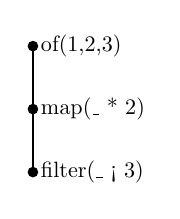
\begin{tikzpicture}[->,>=stealth',shorten >=1pt,auto,node
    distance=1.5cm,
                    semithick,scale=0.8, every node/.style={scale=0.8}]
    \tikzstyle{every state}=[] \filldraw (0,2) circle (2pt) node[right]
    {of(1,2,3)} -- (0,1) circle (2pt) node[right] {map(\_ * 2)} -- (0,0)
    circle (2pt) node[right] {filter(\_ < 3)};
\end{tikzpicture}

	\caption{Simplified graph of Figure \ref{chaincreate}}
	\label{fiddlesimple}
\end{figure}

\begin{figure}[ht]
	\centering
	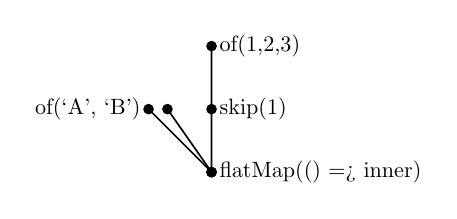
\begin{tikzpicture}[->,>=stealth',shorten >=1pt,auto,node
    distance=1.5cm,
                    semithick,scale=0.8, every node/.style={scale=0.8}]
    \tikzstyle{every state}=[] \filldraw (0,2) circle (2pt) node[right]
    {of(1,2,3)} -- (0,1) circle (2pt) node[right] {skip(1)} -- (0,0)
    circle (2pt) node[right] {flatMap(() => inner)};

    \filldraw (-1,1) circle (2pt) node[left] {of(`A', `B')} -- (0,0)
    circle (2pt) node[right] {};

    \filldraw (-0.7,1) circle (2pt) node[left] {} -- (0,0) circle (2pt)
    node[right] {};

\end{tikzpicture}

	\caption{Simplified graph of Figure \ref{chainhigher}}
	\label{fiddlehigher}
\end{figure}

\paragraph{Layout} Layout is used to add extra meaning to the graph. If multiple subscriptions on the same Observable are created, multiple flows are kept in the graph and they are bundled together in the resulting layout. This is designed to help developers find related flows. Also it is easy to see that for example an Observable is reused many times, hinting a possible performance improvement by sharing the computation (Rx has special \code{share}-operators to multicast). The layout is based on StoryFlow~\cite{liu2013storyflow}, which employs a hierarchical clustering before ordering the graph in a way to reduce crossings. Where StoryFlow clusters on physical character location we cluster flows per Observable. Furthermore, StoryFlow supports interactivity in various layout stages of which we use the algorithms for \emph{straightening} and \emph{dragging} to support selecting a specific flow, which is then highlighted, straightened and positioned at the right in order to match the marble diagram, shown for the current highlighted flow.

\paragraph{Color} Coloring the nodes can be used to identify the same Observable in multiple places in the graph, as Observables can be reused in different places of the stream.

\subsection{Dynamic Marble Diagrams}
In contrast to the original diagrams (Section \ref{marblediagram}) we use dynamic diagrams which update live when new events occur and are stacked to show the data in the complete flow. This allows the developer to trace a value back through the flow, a debug operation which is impossible using a classic debugger. Handcrafted marble diagrams can use custom shapes and colors to represent events, but for the generic debugger we use only three shapes: next-events are a green dot, errors a black cross, completes a vertical line, as shown in Figure~\ref{screenshot-mergeAll}. For our generic debugger it is unfeasible to automatically decide which properties (content, shape and color) to apply to events, as the amount of events and distinguishing features might be unbounded. Instead the event values are shown upon hovering.

\subsection{Architecture}
To support the visualization, we design a debugger architecture consisting of 2 components:

The \textbf{Host instrumentation} instruments the Rx library to emit useful execution events. Depending on the language and platform, specific instrumentation is required. Output of the instrumentation is a platform and language independent graph like Figure \ref{chainhigher}. By splitting the instrumentation, the debugger can be used for the complete ReactiveX family of libraries by only reimplementing the first component. The communication protocol for the instrumentation is shown in Table \ref{protocol}. 

The \textbf{Visualizer} takes the initial graph and simplifies it into a Data Flow Graph. Then it lays out the Data Flow Graph and provides the debuggers User Interface. By separating the visualizer, we can safely export generated graphs and visualize them post mortem for example for documentation purposes.

The components can run in their own environment. The instrumentation must run inside the host language, while the Visualizer can use a different language and platform.

\begin{figure*}
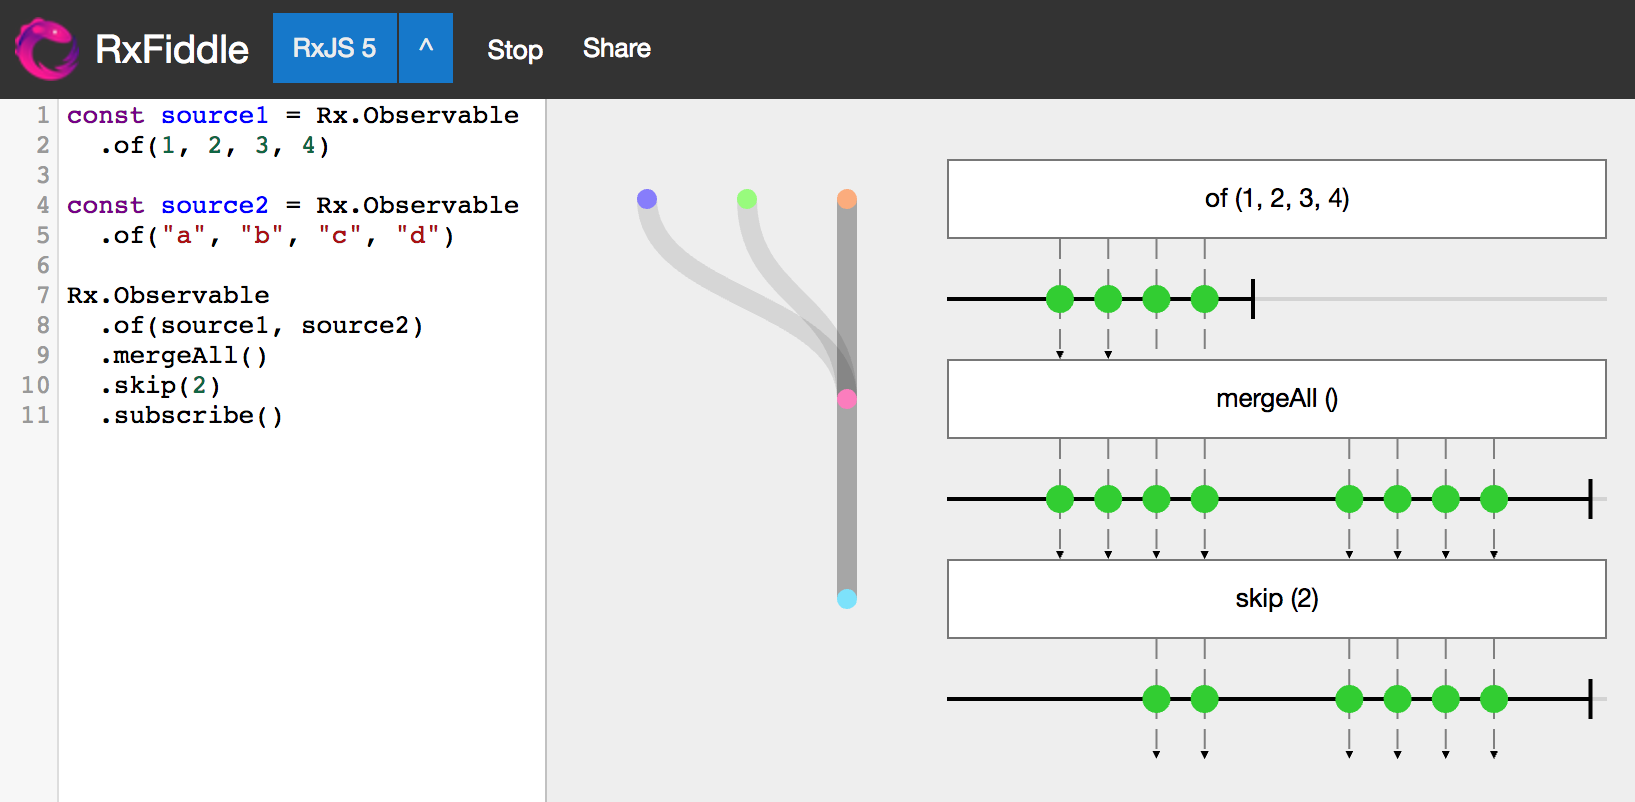
\includegraphics[width=\textwidth]{{images/screenshot.mergeAll.crop}.png}
\caption{Screenshot of \href{http://rxfiddle.net/\#type=editor&code=Y29uc3Qgc291cmNlMSA9IFJ4Lk9ic2VydmFibGUKICAub2YoMSwgMiwgMywgNCkKCmNvbnN0IHNvdXJjZTIgPSBSeC5PYnNlcnZhYmxlCiAgLm9mKCJhIiwgImIiLCAiYyIsICJkIikKClJ4Lk9ic2VydmFibGUKICAub2Yoc291cmNlMSwgc291cmNlMikKICAubWVyZ2VBbGwoKQogIC5za2lwKDIpCiAgLnN1YnNjcmliZSgp}{RxFiddle.net}}
\label{screenshot-mergeAll}
\end{figure*}

\begin{table*}[t]
\centering
\resizebox{\textwidth}{!}{%
\begin{tabular}{|l|l|}
\hline
addObservable(id, sourceIds)                   & Adds a Observable node, with zero or more source Observable's                                                                                                                      \\ \hline
addObserver(id, observableId, destinationId)   & \begin{tabular}[c]{@{}l@{}}Add a Observer, observableId denotes the Observable it subscribed to, \\ optional destinationId adds an edge to the destination Observer\end{tabular}   \\ \hline
addOuterObserver(observerId, outerDestination) & \begin{tabular}[c]{@{}l@{}}Create a special edge between an existing Observer and the higher order \\ destination Observer\end{tabular}                                            \\ \hline
addEvent(observerId, type, optionalValue)      & \begin{tabular}[c]{@{}l@{}}Add an event to the Observer denoted by observerId, of type (next, error, complete), \\ optionally with a value (for next / error events).\end{tabular} \\ \hline
addMeta(id, metadata)                          & Add meta data such as the method call which created an Observable.                                                                                                                 \\ \hline
\end{tabular}%
}
\caption{Instrumentation protocol}
\label{protocol}
\end{table*}

\subsection{Implementation}
To validate the design and to provide an implementation to the developer community we created \url{RxFiddle.net}. The RxFiddle project is a reference implementation of 
our reactive debugger design. Besides the visualizer, the website also contains a code editor for JavaScript code with sharing functionality, for developers to share snippets with their peers, as shown in Figure \ref{screenshot-mergeAll}. In this section we will explain different parts of the implementation. For RxFiddle, we initially focused on RxJS (JavaScript).

\paragraph{Instrumentation}
With JavaScript being a dynamic language, we use a combination of prototype patching and Proxies\footnote{\url{https://developer.mozilla.org/docs/Web/JavaScript/Reference/Global_Objects/Proxy}} to instrument the RxJS library: the Observable and Observer prototypes are patched to return Proxies wrapping the API method calls. The instrumentation passes every method entry and method exit to the Linking-step.

\paragraph{Linking}
Here, we distinguish between method calls from the different phases (Section \ref{nutshell}). From the assembly phase, we detect when Observables are used as target or arguments of a call or as return value, and create a graph node for each detected Observable. We add an edge between the call target \& call arguments and returned Observables, denoting the `source'-relation. Also, we tag the returned Observable with the call frame information (time, method name, arguments). In the subscription phase we detect calls to the \code{subscribe}-method: the destination Observers are passed as arguments, so we create the graph nodes and save the relation as an edge. In the runtime phase we detect `next', `error' and `complete' calls on Observers and add these as meta data to the Observer nodes.

\paragraph{Graph Loggers}
From the Linking-step the graph mutations are streamed to the environment of the visualizer, where the graph is rebuild. Depending on the host language a different protocol is used: RxFiddle's code editor executes the code in a Worker\footnote{\url{https://developer.mozilla.org/docs/Web/API/Worker}} and transmits events over the postMessage protocol, while RxFiddle for Node transmits over WebSockets. Being able to support multiple protocols increases the possible use cases, ranging from the code editor for small programs, to the Node plugin for server applications, to Chrome DevTool extensions\footnote{\url{https://developer.chrome.com/extensions/devtools}} for web applications.

\paragraph{Visualizer}
The visualizer receives the current state in the form of a graph from the Logger. It then uses the Observers in the graph to create the Data Flow Graph (DFG). 
To layout the DFG using StoryFlow~\cite{liu2013storyflow} we first rank the graph using depth first search, remove slack and reverse edges where necessary to create a directed acyclic graph. We then add dummy nodes to replaces long edges with edges spanning a single rank. Finally we order and align the nodes in the ranks assigning coordinates for the visualization. It is important that layout is fast, as it runs every time the DFG is changed. To render the Marble Diagrams the flow to and from the selected Observer is gathered by recursively traversing the graph in the direction of the edges, respectively the reversed direction.


\section{Evaluation}
\label{section-evaluation}

In this section we evaluate our ideas about the debugger that we designed, by answering RQ3. 
The goal of the experiment is to measure the \textit{time} required to solve programming problems~\cite{ko2015practical}. We use time instead of correctness as it matches debugging better: a developer needs to continue debugging \textit{until} he finds an explanation or a solution to his problem. During debugging incorrect assumptions can be tested and corrected. We measure the time from the moment the participant receives the question until the correct answer is given. Participants use either the built-in Chrome Browser debugger (group `Console') or - the treatment - our RxFiddle debugger (group `RxFiddle'). This single alternative debugger together with the experiment UI (which acts as a small IDE) offers all the debugging capabilities subjects of our preliminary interview (RQ1) reported to use.

The experiment consists of a questionnaire, a warm-up task and 4 programming tasks, all available in a single in-browser application. The questionnaire contains questions regarding age, experience in several programming languages and several reactive programming frameworks. We use this self estimation as a measurement of skill instead of a pretest, since it is a faster and better estimator~\cite{kleinschmager2011rate,feigenspan2012measuring,siegmund2014measuring}. The warm-up program is situated in the same environment as the programming problems and contains several tasks designed to let the participants use every control of the test environment. The first 2 programming problems require the participants to obtain an understanding about the behavior of the program and report the findings. The last 2 programming problems contain a program with a bug. The participants are asked to find the event that lead to the bug in the third problem and to identify and propose a solution in the fourth problem. The first 2 problems are synthetic examples of two simple data flows, while the latter contain some mocked (otherwise remote) service which behaves like a real world example.

We use a between-subjects design for our setup. While this complicates the results - subjects have different experience and skills - we can not use a within-subjects design as it would be impossible to control for the learning effect incurred when asking subjects to perform survey questions with and without the tool. This also allows us to restrict the amount of tasks to incorporate in the experiment, requiring less time of our busy subjects.

%\todo{Discuss guidelines defined in ko2015practical~\cite{ko2015practical}}

\subsection{Context}
The experiment was run in a controlled and an online setting.
The controlled experiment was conducted at a Dutch software engineering company. Subjects are developers with several years of programming experience, and range from little to no experience with RP to many years of experience (Figure \ref{fig-experience}). Some of the subjects had already used RxFiddle, forming a potential threat to validity. As we do not try to measure the effect of learning a new tool, but rather using a tool after learning to use it, we explained RxFiddle in the introductory talk and added the warm-up question to get every participant to a minimum amount of knowledge about the debugger at hand.

The online experiment was announced by several core contributors to RP libraries on Twitter and via various other communication channels. Subjects to the online experiment took the test at their own preferred location and have possibly very different backgrounds. Several short video tutorials were created and included in the online experiment to introduce the participants to the debug tool available to them and the tasks they needed to fulfill.

\begin{figure}[h]
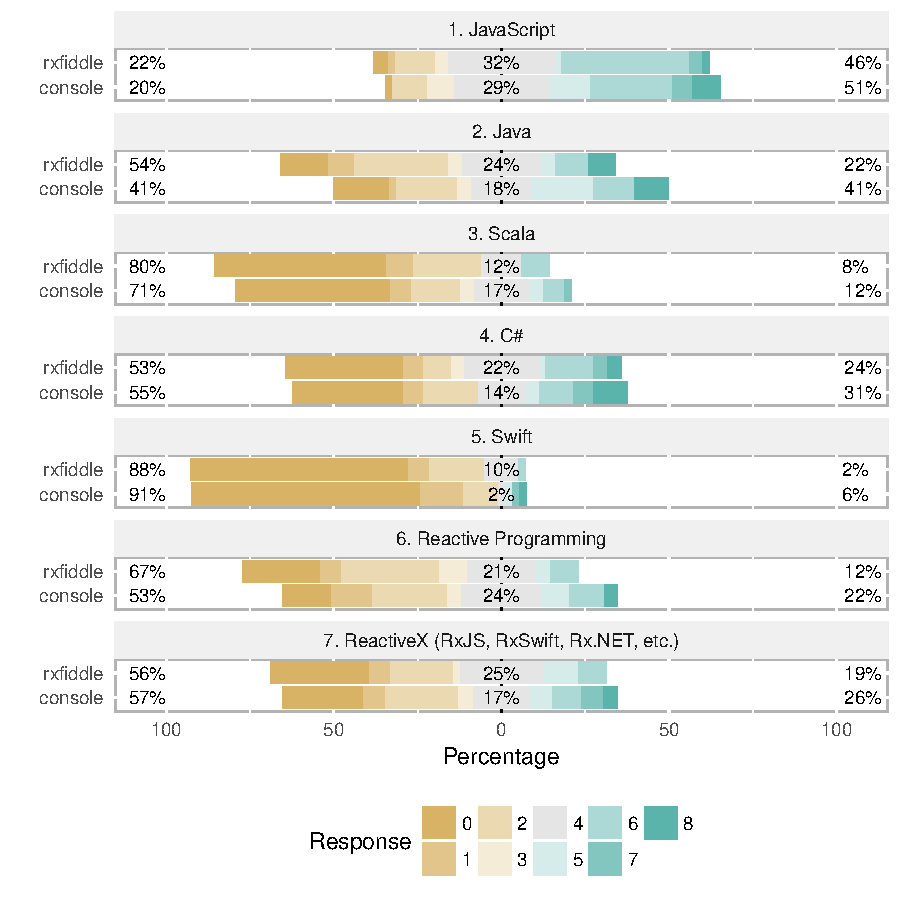
\includegraphics[width=\columnwidth]{images/experience.pdf}
\caption{Experience in various programming languages, 9-point Likert scale}
\label{fig-experience}
\end{figure}


\subsection{Results}
The online experiment was performed outside of our control, and some participants quit the experiment prematurely. In total we had 105 subjects starting the survey, of those 93 completed the preliminary questionnaire, and 84, 71, 65, and 56 subjects started respectively T1, T2, T3 and T4. All of the subjects in the offline setting started all tasks. Figure~\ref{fig:resultPerTask} shows the outcome of the tasks; in the remainder of this section consider only the outcomes marked as ``Correct''.

\begin{figure}[t]
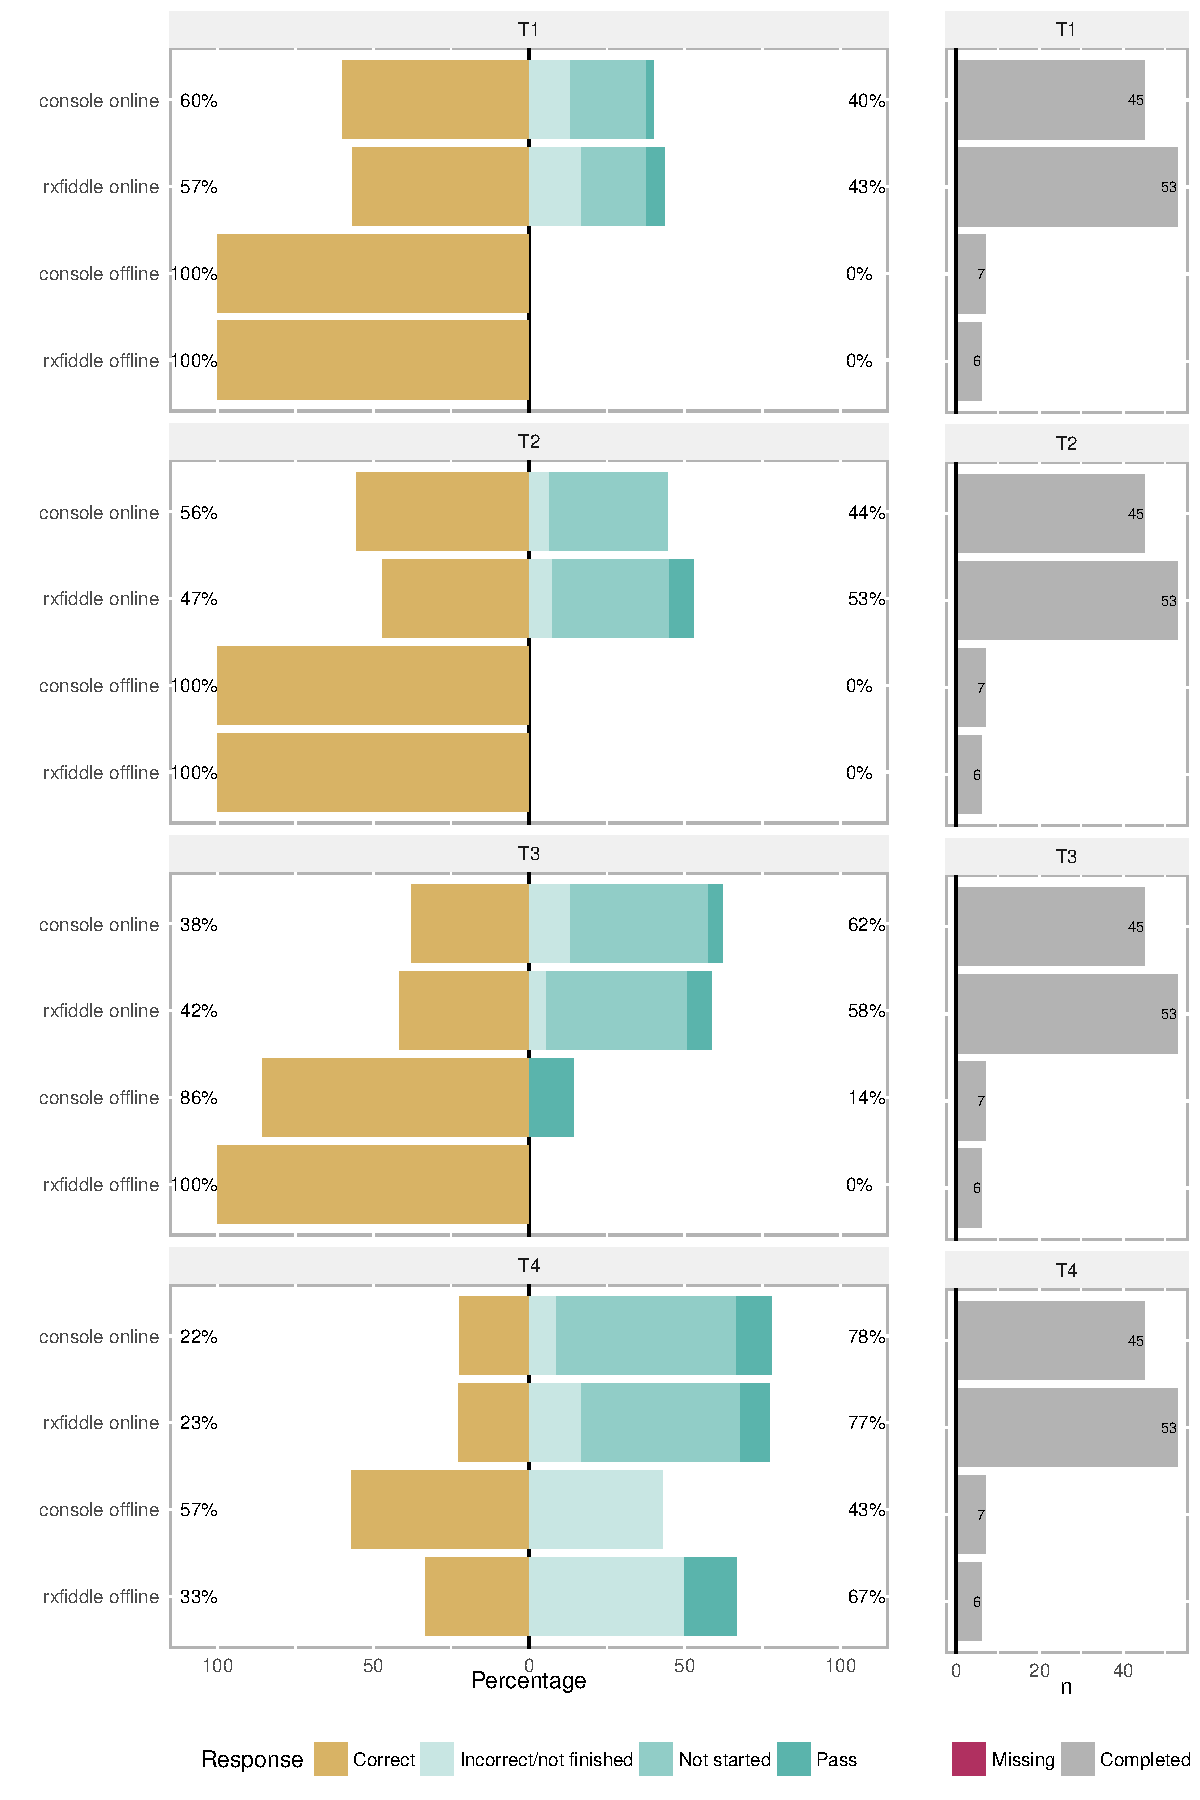
\includegraphics[width=\columnwidth]{images/resultPerTask.pdf}
\caption{Task outcome per group (RxFiddle/Console) and environment (online/offline)}
\label{fig:resultPerTask}
\end{figure}

\paragraph{Overall}
Figure \ref{fig:timePerTask} shows the time until the correct answer was given per task. Here we consider both the results from the offline experiment as the online experiment. We make no assumptions about the underlying distribution so we perform a non-parametric Wilcoxon Mann-Whitney U test (\textit{$H_0$: times for the Console group and RxFiddle group are drawn from the same population}) to see if the differences are significant, and a Cliff's delta test for ordinal data to determine the effect size.

\begin{centering}
% \begin{table}[]
% \centering
% \caption{My caption}
%\label{my-label}
\begin{tabular}{llllll}
\hline
            & \textbf{$n_1$} & \textbf{$n_2$} & \textbf{W} & \textbf{p-value} & \textbf{Cliffs $\delta$} \\ \hline
\textbf{T1} & 26                      & 30                       & 343        & 0.448           & 0.121     \\
\textbf{T2} & 29                      & 27                       & 362        & 0.637           & 0.0754    \\
\textbf{T3} & 22                      & 24                       & 100        & 0.000186        & 0.621     \\
\textbf{T4} & 15                      & 12                       & 86         & 0.867           & 0.0444    \\ \hline
\end{tabular}
% \end{table}
\end{centering}

For tasks T3 we can reject $H_0$ with high significance ($p < 0.05$), \emph{the RxFiddle group is faster}.
For the tasks T1, T2 and T4 we can not reject $H_0$ ($p > 0.05$), meaning the \emph{RxFiddle group and Console group perform or could perform equally}.

\begin{figure}[t]
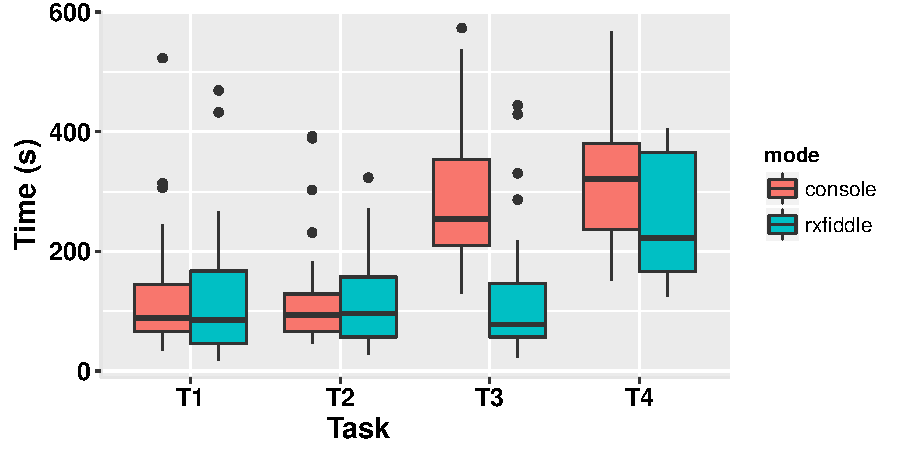
\includegraphics[width=\columnwidth]{images/timePerTask.pdf}
\caption{Time until correct answer per task, overall}
\label{fig:timePerTask}
\end{figure}

\paragraph{Control for experience}
To investigate this further, we split the results for different groups of subjects, as shown in Figure \ref{fig:timePerTaskSplit} in the Appendix.
When we control for the self-assessed Rx experience (splitting at the median value; greater than ``Beginner''-level) we see bigger differences for all tasks for groups with more experience, as shown in Figure~\ref{fig:timePerTaskRx} and the following table.

\begin{centering}
\begin{tabular}{llllll}
    \hline
                & \textbf{$n_1$} & \textbf{$n_2$} & \textbf{W} & \textbf{p-value} & \textbf{Cliff's $\delta$} \\
    \hline
    \textbf{T1} & 16             & 17             & 105        & 0.276            & 0.228                     \\
    \textbf{T2} & 14             & 13             & 99         & 0.720            & -0.0879                   \\
    \textbf{T3} & 10             & 11             & 10         & $7.88e^{-4}$     & 0.818                     \\
    \textbf{T4} & 8              & 7              & 13         & $9.34e^{-2}$     & 0.536                     \\
    \hline
\end{tabular}
\end{centering}

\begin{figure}[t]
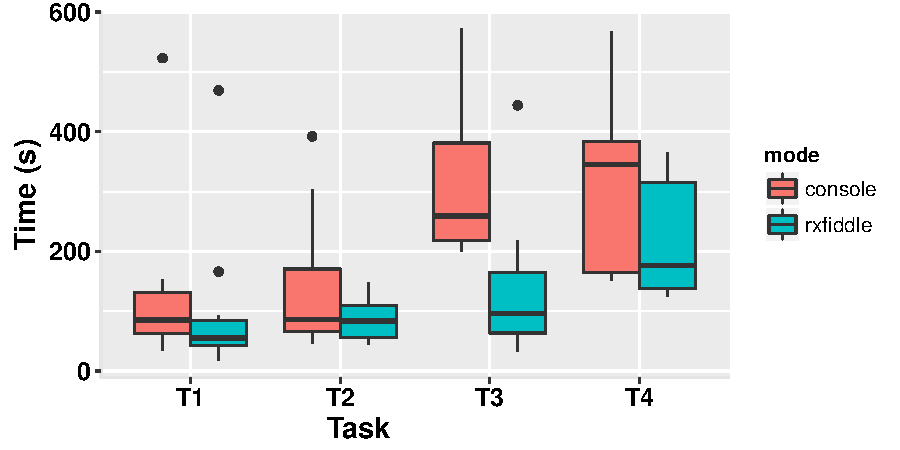
\includegraphics[width=\columnwidth]{images/timePerTaskRx.pdf}
\caption{Time until correct answer per task, for subjects with more than ``Beginner''-level of experience with Rx}
\label{fig:timePerTaskRx}
\end{figure}

Still, for tasks T1, T2, and T4 we can not reject $H_0$, but the results are more significant comparing only experienced subjects.


\section{Discussion} We now discuss our main findings, how RxFiddle
resolves the debugging problem of Rx, and contrast our design to other
design choices and possibilities of future work.

\subsection{Main results}
\paragraph{Quick and dirty debugging} Through interviews and literature
we establish that current debugging practices for RP consist mostly of
\printfdebugging{}.  The shortcomings of this method were evident from
the interviews:  it works reliably only for synchronous execution or
small amounts of events being logged, otherwise overview is lost.
Furthermore the time-context of events and dependency-context of flows
are not available using this method.  We attribute the prevalence of
\printfdebugging{} to this \emph{``quick and dirty''} method being
available in every language and on every platform, without a viable
alternative.

\paragraph{Improved context:  being complete, disposing doubts} With our
design and complementary implementation we show that the abstract model
of RP is suitable for visualization on two levels:  overview and detail.
On the overview level, we complement the dependencies visible in source
code with a graph of the resulting structure, showing the run-time
effect of certain operators on the reactive structure.  On the detail
level we add the time-context, by showing previous values on a
horizontal time line, and the dependency-context, by showing input and
output flows above and below the flow of interest.  While the results of
our evaluation could be observed as a negative, RxFiddle is a new tool,
where subjects have only just been exposed to the tool and received only
a short training.  We expect that by designing a debugger model so close
to the actual abstractions, our debugger works especially well for users
with some knowledge of these abstractions; while only T3 shows better
performance with high significancy, we observe slightly better results
when controlling for experience.  Future research might investigate the
effect of experience in more detail, including the use of more
complicated tasks, with larger samples.

In the presented research, we did not perform tests with subjects using
their own code.  However, during piloting and after the release of
RxFiddle we received positive feedback regarding the completeness of the
visualization.  As one user put it, \emph{``by using RxFiddle when
learning and understanding what RxJS does in our project, I have a
feeling of improved control over our Observables, Subscriptions and the
reactive parts of our app''}.  Specifically the life-cycle events, which
are generally hard to debug using \printfdebugging{}, are more clear:
\emph{``Initially we were reluctant to manually subscribe, but after
seeing that `complete' often triggers a `dispose', the team became more
confident to sometimes use \code{subscribe()} directly''}.  Future
research might address this by designing experiments specifically using
the users own code.

%%%%%%%%%%%%%%%%
% Quotes:
% ``the experience helped me understand what a specific operator was doing and how it was messing up my code.''
% `` Dat was de ervaring die ik net beschreef en die kwam direct voort uit wat wij keer hadden besproken dat `.share()` iets complexer is dan dat wij (als team) hadden gedacht en dat de effecten van hem twee keer gebruiken nogal, ongewenst waren. Dat hadden we op geen manier kunnen debuggen zonder RxFiddle, want met een `console.log()` kan je dat niet checken''.
% ``Wij waren vroeg in het project een beetje huiverig voor `subscribe()` en door RxFiddle zagen we dat een `onComplete()` ook een `unsubscribe()` triggert, in veel gevallen. En dat maakte het team iets geruster om hier en daar een `subscribe()` te gebruiken.''
% ``Door m’n ervaringen met onder andere RxFiddle ten tijde van het leren en begrijpen van wat RxJS in ons project doet, heb ik het idee nu meer grip te hebben op onze Observables, Subscriptions en de Reactive delen van onze applicatie.''

%%%%%%%%%%%%%%%%% OLD


\subsection{Implications}
The developers using Rx in practice now have an alternative to \printfdebugging{}. 
We recommend developers to try RxFiddle on their codebase to better understand the reactive behavior of their applicatoin, 
and potentially detect (performance) bugs they are not aware of.
At least example of this has already occurred in practice:
we helped one of our interview subjects with a bug\footnote{\url{https://github.com/ReactiveX/rxjs/pull/2662}} in the \code{groupBy} implementation of RxJS,
which resulted in retention of subscriptions, increased memory usage and finally an out-of-memory exception;
the bug was detected in practice and required extensive amount of debugging involving the NodeJS debugger to trace down, 
but could be validated quickly by examining the life-cycle events in RxFiddle.

Contributors of RP libraries should use tools like the RxFiddle visualizer in documentation to provide executable samples,
which would allow for a better learning experience, 
and at the same time introduces novice developers to other ways of debugging than \printfdebugging{}.


\paragraph{Graph scalability}
Debugging large reactive systems over longer periods of time can result in significantly larger Observable graphs and Marble Diagrams than currently evaluated. During tests of RxFiddle with larger applications like RxFiddle itself and an existing Angular application the graph became too large to render in a reasonable amount of time. Besides rendering performance, a potentially even bigger issue is with communicating large graphs to the developer. We propose several extensions to RxFiddle to remedy this issue: (1) pruning the graph of old flows to show only the active flows, (2) bundling flows that have the same structure and only rendering a single instance offering a picker into the flow of interest, (3) collapsing certain parts of the graph that are local to one source file or function, (4) adding search functionality to quickly identify flows by operator or data values, (5) support navigation between code \& graph.

\paragraph{Marble Diagram scalability}
Furthermore we think that while Marble Diagrams are useful for small to medium amount of events ($< 20$), both better performance and better functionality would be achieved by providing a different interface for high volume flows. Above a certain threshold of events this high volume interface could be the default, offering features like filtering, watch expressions (to look deeper into the event's value), and advanced features like histograms \& FFT.

\paragraph{Breakpoints}
\label{breakpoints}
Setting traditional breakpoints in a reactive program stops the system from being reactive, and therefore can change the behavior of the system. This was our reason not to include breakpoints in RxFiddle. However, the behavior of breakpoints is twofold: they allow us to modify the application state by interacting with the variables in scope, but they also provide a way to be notified of an event occurrence. While the first is arguably not desirable for reactive systems, the notification property might be a good addition to RxFiddle. BIGDEBUG~\cite{Gulzar2016}, a debugging solution for systems like Spark~\cite{zaharia2012resilient}, introduces \textit{simulated breakpoints} for this purpose. When a simulated breakpoint is reached, the execution resumes immediately and the required lineage information of the breakpoint is collected in a new independent process. Implementing this for RxFiddle is a matter of creating the right UI as the required lineage data is already available.


\section{Threads to validity}

\todo{look at \url{http://ieeexplore.ieee.org/document/7476654/\#full-text-section}}
\todo{look at Contributors paper of Gousios}

\textbf{Subjects.} The online experiment was open to anyone who wanted to participate. As a result a mixed group of developers took part, even those without Rx experience. The total amount of participants filling in the preliminary survey for the experiment was larger than the group finishing the experiment and some participants stopped during the tasks. We only consider results from fully completed tasks.

\textbf{Tasks.} The experiment consists of 2 small and 2 medium tasks, so the results of the experiment might not necessarily generalize to debugging RP in practice with larger systems. For larger tasks the effect of using the debugger could be bigger and therefore be better measurable. Still, we chose for these smaller tasks: in the limited time of the subjects they could answer only so many questions. With the limited amount of time available, we still show that a significant speed-up can be achieved in some cases. We leave it for future work to extend the experiment to include larger systems.


\section{Related Work}

\paragraph{RP Debugging} 
REScala~\cite{salvaneschi2014rescala} is a RP library for Scala, based on Scala.React. 
Recently a debugger model was created for REScala, called ``RP Debugging''~\cite{salvaneschi2016debugging}, 
featuring a dependency graph visualization, breakpoints, a query language and performance monitoring.
The debugger fully integrates with the Eclipse IDE and the Scala debugger facilities, 
creating a (Scala) developer experience and a feature RxFiddle currently can not offer: reactive breakpoints. 
However breakpoints are arguably not as useful as ``simulated breakpoints'' (Section \ref{breakpoints}, \nameref{breakpoints}).
Furthermore, our debugger design support multiple languages, and works outside of the IDE,
in the browser environment and/or connecting to a production system.
Rx has different reactive semantics and a more powerful, but also more extensive API, which includes operators acting in the time domain (\code{delay}, etc.).
Therefore, we argue that seeing the many values in a flow over time is very valuable; 
RP Debugging shows the latest values at the selected time.

\paragraph{RP Visualization} 
RxMarbles~\cite{rxmarbles} visualizes single Rx operators, for the purpose of learning and comprehension.
Users can modify the diagrams by dragging the events and instantly see the changes reflected in the output.
By using specific precoded inputs and timings the essence of the operator is made clear.
In the soon to be released RxViz~\cite{rxviz}, 
Moroshko takes a similar approach, but uses code instead of prepared inputs.
Where RxMarbles is limited to non higher order flows, RxViz subscribes to all inner Observables when it detects a higher order Observable showing them concurrently.
In contrast to our work, these tools focus only on learning single operators.

\paragraph{Omniscient Debugging} Omniscient debuggers~\cite{pothier2009back} are ``all-knowing debuggers'', 
that trace, store and query all events in a program execution.
When storing vasts amount of program execution information, performance and efficiency becomes very much a problem and research in omniscient debuggers focus on this specifically.
We also trace events of the entire execution, however in contrast to omniscient debuggers we only store trace events regarding RP data flows.
The RP semantics allow us to create future optimizations, for example retaining only the active flow structure, while the flow's data is kept in a rolling buffer.

\paragraph{Dynamic Analysis.}
The study of program execution is called ``dynamic analysis''~\cite{cornelissen2009systematic}.
In most cases dynamic analysis involves a \textit{post mortem} analysis, 
where first the program is run, collecting an execution trace, and then the trace data is analyzed to create a visualization.
The various derived visualizations, like class and instance interaction graphs, function invocation histories~\cite{lange1995program}, invocation views and sequence diagrams~\cite{cornelissen2008execution} show the possibility to use trace information for debugging.
Arguably an on-line analysis is more useful for debugging than the standard post mortem analysis. Reiss mentions the compromises that have to be made to make an on-line analysis~\cite{reiss2006visualizing}: 
reduced tracing is required to not slow down the system (known as the observer-effect) and
fast analysis is required to lower the cost of getting to the visualization, to not discourage the users.
In our design, we handle the same compromises as they are relevant for RP debugging too, and our JavaScript trace implementation bears resemblance to that of Program Visualiser~\cite{lange1995program}.

% \todo{
% \begin{enumerate}
%  \item Cornelissen, TU Delft, survey on Program Compr. through Dynamic Analysis
%  		lists limitations: 
% 		   - incompleteness, only part of domain
% 			 - which scenarios to analyse
% 			 - scalability (wrt human cognitive load) 
% 		 	 - observer effect (multi-threaded, realtime) changes execution
% \end{enumerate}
% }

% \todo{
% \begin{enumerate}
% 	\item Atlas (2014): rich graph representation, can be used to build call graphs, dataflow graphs, dependency graphs
% %	\item RP debugging (2016, Guido): REScala, data flow graph, breakpoints
% %	\item BIGDEBUG Spark debugging (2017): data flow graph, non-pausing simulated breakpoints, data provenance
% \end{enumerate}
% }

% \textbf{Tracing \& Automated visualization for comprehension}
% \todo{
% \begin{enumerate}
%  \item Lange 1995, Program Visualizer for C++
%  \item story flow: visualize stories over time, comprehending relations, interactive visualization
%  \item Weck \& Tichy, Visualizing Data-Flows in Functional Programs
%  \item Srinivasan, ICPC16, ``Case Studies of Optimized Sequence Diagram for Program Comprehension", Texas A\&M Univerity
% %  \item Misha Moroshko (Facebook) Rx visualization
% \end{enumerate}
% }

\paragraph{Understanding Debugging}
Debugging for general purpose languages revolves around 
attaching a debugger,
stepping through the code, 
attaching code or data breakpoints, 
navigating along different calls in the call stack and 
examining variables and results of expressions~\cite{Spinellis2017}.
However, existing research measuring how these different tasks are part of the developers work day found that 
while developers spend much time on comprehending code they do not spend much time inside the IDE's debugger~\cite{minelli2015know}.
Beller et al.~\cite{beller2017behavior} found that only 23\% of their subjects actively use the IDE's debugger,
with the most common action being adding breakpoints, followed by stepping through code.
The automated tooling of these studies did not measure different kinds of debugging other than using the IDE provided tools, 
however Beller's survey indicates that 71\% also uses \code{printf} statements for debugging.
No indication was given of any RP language and libraries used by the subjects in the study, 
but the observation that \printfdebugging{} is common matches our experience with debugging reactive programs.

% What comprises debugging?
% \item Maybe Zeller / Spinellis?

% \item Petrillo, ``Towards Understanding..." e.g. Swarm debugging
% \item Minelli (know what you did last summer)
% \item Moritz (watchdog 2.0)

\paragraph{Debugging for Program Comprehension}
Both debugging and comprehension are processes in the work of programmers.
Initially comprehension was seen as a distinct step programmers had to make
prior to being able to debug programs~\cite{katz1987debugging}, 
but this distinction is criticized by Gilmore saying we must view 
``debugging as a design activity''~\cite{gilmore1991models}, 
part of creating and comprehending programs. 
Maalej et al.~\cite{Maalej2014} interviewed professional developers 
and found that developers require runtime information to understand a program,
and that debugging is frequently used to gather this runtime information.
This supports our view that debugging is not only used for fault localization,
but also for comprehension.

% \item Katz, distinct step
% \item Gilmore, comprehension + debugging == linked
% \item Maalej: professionals, avoid deep comprehension, sharing knowlegde


\section{Conclusion}
Observing the current debugging practices, this work shows the prevalent method for RP debugging of \printfdebugging{}.
To provide a better alternative, we have created a debugger design for RP and presented the RxFiddle implementation, a RP debugger for RxJS, which allows developers to: (1) gain a high-level overview of the reactive data flow structure, (2) investigate the values and life-cycle of a specific data flow, at run-time.

Through an experiment we show that RxFiddle is an viable alternative for traditional debugging and in some cases outperforms traditional debugging in terms of time spent. There are several promising directions for improving our current design.
Specifically scalability could be improved and different edge visualizations could be explored, to improve the usability of the tool. Furthermore, by leveraging already captured meta data about timing of events, even more insight could be provided. At the implementation level, we plan to extend RxFiddle to other members of the Rx-family of languages.

In this paper, we make the following concrete contributions:
\begin{itemize}
\item[(1)] Design of a RP debugger
\item[(2)] The implementation of the debugger for RxJS, and the service RxFiddle.net, a platform for the debugger in an online environment with code sharing functionality.
\end{itemize}

The debugger and the platform are open source and are available online at~\cite{rxfiddle-doi}.


\AtNextBibliography{\small} \printbibliography

%% Use letters for the chapter numbers of the appendices.
\appendix

\begin{figure*}[ht]
\centering
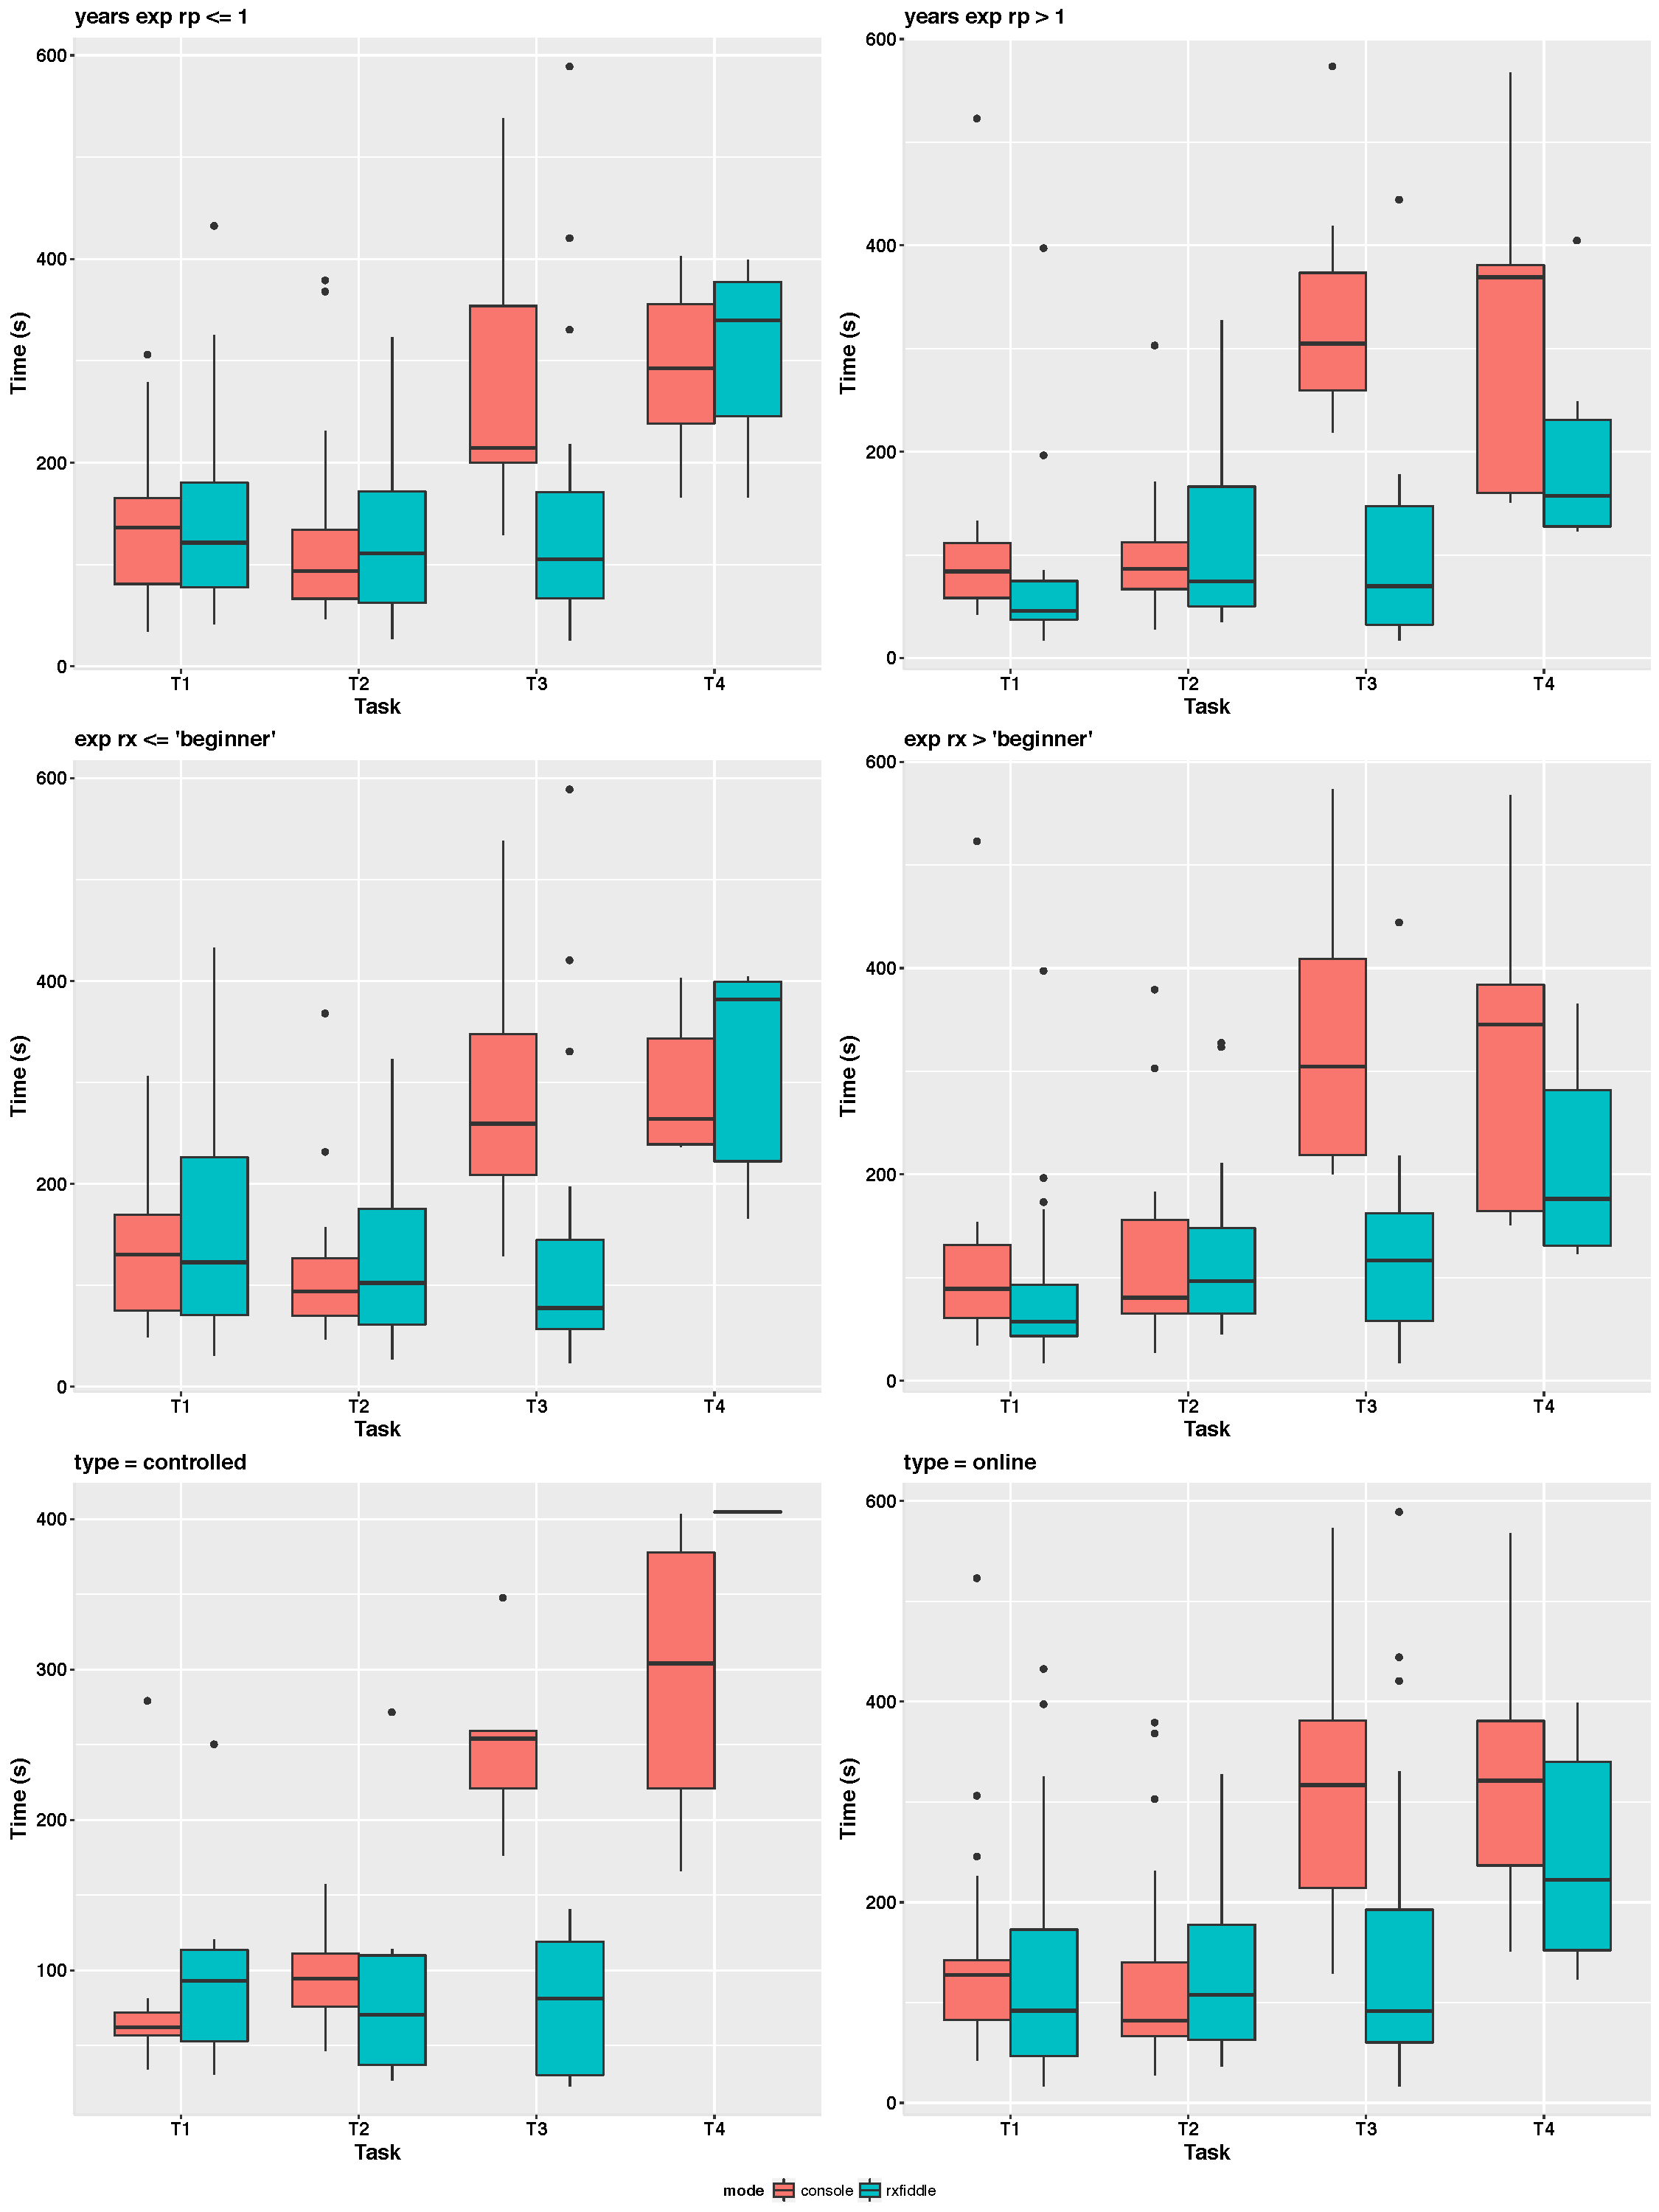
\includegraphics[width=0.9\textwidth]{images/timePerTaskSplit.pdf}
\caption{Time until correct answer per task, split in various groups}
\label{fig:timePerTaskSplit}
\end{figure*}


\end{document}
